\documentclass[]{article}

% Imported Packages
%------------------------------------------------------------------------------
\usepackage{amssymb}
\usepackage{amstext}
\usepackage{amsthm}
\usepackage{amsmath}
\usepackage{enumerate}
\usepackage{fancyhdr}
\usepackage[margin=1in]{geometry}
\usepackage{graphicx}
\usepackage{extarrows}
\usepackage{setspace}
%------------------------------------------------------------------------------

% Header and Footer
%------------------------------------------------------------------------------
\pagestyle{plain}  
\renewcommand\headrulewidth{0.4pt}                                      
\renewcommand\footrulewidth{0.4pt}                                    
%------------------------------------------------------------------------------

% Title Details
%------------------------------------------------------------------------------
\title{SE 3A04: Software Design II -- Large System Design}
\author{Team 11}
\date{}  
                             
%------------------------------------------------------------------------------

% Document
%------------------------------------------------------------------------------
\begin{document}

\maketitle
\begin{center}
\hrule
	\vspace{0.2in}
\huge AudioVal.ly
	\vspace{0.05in}
\hrule
	\vspace{0.2in}
\huge  Software Requirements Specification
	\vspace{0.2in}

\large February 9, 2018
\\
	\vspace{1in}
			\large Team 11
\end{center}
\begin{minipage}[c]{\linewidth}
%\fontsize{14pt}{25pt}\selectfont
			\large
			\centering
			\begin{tabular}{l c c}
				Baltej Toor & 1413818 & toorbs \\
				Brandon Roberts & 400018117 & roberb1 \\
				Corey Szeto & 400025728 & szetoc \\
				Jiahong Dong & 1452923 & dongjh \\
				Puru Jetly & 1417837 & jetlyp \\
			\end{tabular}
\end{minipage}	
\newpage

\tableofcontents
\newpage
\section{Introduction}
\label{sec:introduction}
% Begin Section

This section outlines the purpose and scope of the AudioVal.ly; along with definitions, acronyms and abbreviations used within this document; and finally an overview of the contents and organization of this software requirements document.

\subsection{Purpose}
\label{sub:purpose}
This document's purpose is to outline the engineering and business decisions made in the design portion of the AudioVal.ly. This document will be used to maintain a record of project's scope, constraints, assumptions, dependencies, functional requirements, non-functional requirements and any other design decision made over the life of this project.

The target audience for this document are the stakeholders (Dr. Ridha Khedri, Spencer Deevy and Andrew Le Clair ), and any current or future architects, designers and developers of this project.


\subsection{Scope}
\label{sub:scope}
This project will produce the following software product:
\begin{itemize}
  \item Android client application
\end{itemize}

\noindent The aforementioned product perform the following:
\begin{itemize}
  \item Provide users with a graphical client-side application for identifying \textbf{music genres}.
\end{itemize}

This software product will provide a means to identify different \textbf{music genres} of music. Benefits of this include quick access to genre content, efficient management of genre content, portability, and, ease of access to genre content.  The goals of this project include providing users with an easy-to-use interface to quickly identify \textbf{music genres}, and a way to access previously identified \textbf{music genres}.  


\subsection{Definitions, Acronyms, and Abbreviations}
\label{sub:definitions_acronyms_and_abbreviations}
a) Provide the definitions of all terms, acronyms, and abbreviations required to properly interpret the SRS
\begin{description}
 \item [Android] An Unix-based operating system developed by Google Inc. for
    electronic devices including but not limited to touch-enabled
    Smartphones, tablets, and other portable computing devices.
 \item [Music Genre] A term used to describe music that share a certain set of characteristics. Ie. Blues, Rock, Metal, Folk, Country.



\end{description}


\subsection{References}
\label{sub:references}
Currently this section is void.
\subsection{Overview}
\label{sub:overview}
The rest of this documents contains detailed descriptions of this projects design decisions: assumptions, functionality, functional requirements and non-functional requirements.

The other sections are organized into logical subsections. Specifically, Section 2 outlines the overall product description with various subsections. Then the following sections list the requirements. The functional requirements are organized by business events and viewpoints. Non-functional requirements are organized into various subcategories.

\newpage
\section{Overall Description}
\label{sec:overall_description}
% Begin Section
\subsection{Product Perspective}
\label{sub:product_perspective}
% Begin SubSection
Our system is a music \textbf{genre} identifier, for the \textbf{Android} operating system. Other than the \textbf{Android} operating system, the identifying process is not dependant on other existing software solutions. The system simply requires either a built-in or an external microphone to record music for analysis. The application may use other software solutions to supplement functionality, but it will still be able to function independently if those solutions are not available. 
\\
There are many similar existing products, such as Shazam, SoundHound, TrackID and Musixmatch Lyrics that all identify music/songs. Even though they all provide accurate results when identifying the genre of a particular song/music, they do not provide the rationale behind that why the music/song belongs to that particular genre. It is this novel feature that differentiates existing products from \textbf{AudioVal.ly} .

% End SubSection
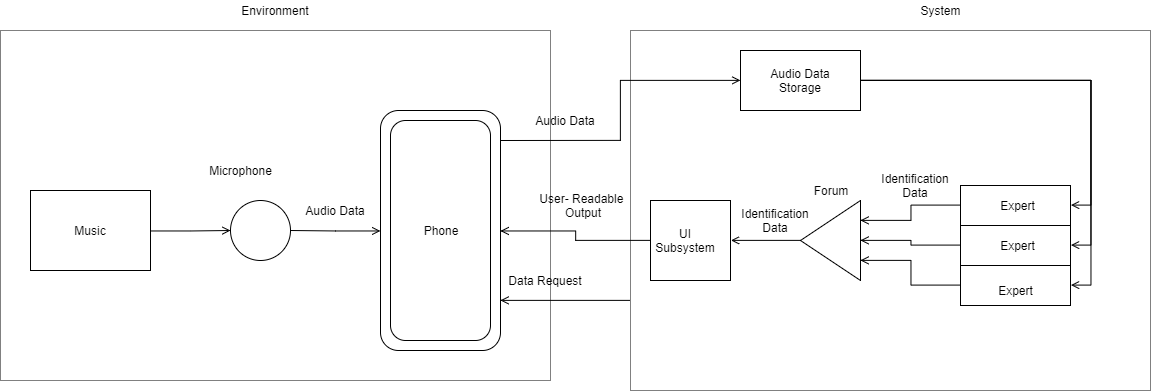
\includegraphics[scale=0.4]{Diag1}

\subsection{Product Functions}
\label{sub:product_functions}
% Begin SubSection
The primary function of our system is to \underline{identify the \textbf{music genre} of music it analyses}. In order to achieve this function, we will have three "experts" to analyse a piece of music that the system recorded and a centralized "Forum" to give the overall result based on the information it gathered from three "experts".

Three experts will process and analyse the music piece from three different aspects (instruments, \underline{lyric themes}, beat per minute) and each report their results to the centralized forum respectively. Once the information has been collected by the centralized forum, the system will resolve any conflicts in case conflicting answers are reported by experts. 

Finally, the identifier will save the \textbf{music genre} it identified and inform the user of what genre it identified the music as belonging to. Besides \textbf{genre}, our addition feature will be also provide the user with the reasons why the system identified the music as beloning to that specific \textbf{genre}.

% End SubSection

\subsection{User Characteristics}
\label{sub:user_characteristics}
% Begin SubSection
Our \textbf{music genre} identifier is intended to be utilised but users who want to know the \textbf{music genre} of the music that is currently being played around them, in this case, potential users could be students in a book store, adults in a bar or elders in a nursing home.

Users will be able to use the \textit{AudioVal.ly} application without any prior training. As long as the user is familiar with navigating the \textbf{Android} operating system they will have no issues with using the application.
% End SubSection

\subsection{Constraints}
\label{sub:constraints}
% Begin SubSection
There is one major constraint, a time constraint. The team has considered many desirable design ideas and extra functionalities that would go beyond the basic requirements. However, since there is a limited and a relatively short amount of time to provide a fully functional product, it makes it infeasible for the team to implement the product it had initially envisioned. As a result, it is more likely that the product will only have basic functionality upon its initial release.
% End SubSection

\subsection{Assumptions and Dependencies}
\label{sub:assumptions_and_dependencies}
% Begin SubSection
The system will be able to perform its task independently assuming that the device has the \textbf{Android} operating system and a microphone. 

The system's functionality is enhanced with the use of existing and external software solutions, but basic functionality of the system is still possible if these dependencies are not available.
% End SubSection

\subsection{Apportioning of Requirements}
\label{sub:apportioning_of_requirements}
% Begin SubSection
N/A
% End SubSection

% End Section

\newpage
\section{Functional Requirements}
\label{sec:functional_requirements}

\begin{enumerate}[{VP}1.]
	\item User 
	\begin{enumerate}[{BE1}.1]
		\item The user wants to identify the genre of a song that is playing [over the radio.]
		\begin{enumerate}
			\item The system shall take audio information from the device’s microphone and store it.
			\item The system shall process stored audio information by using three experts.
			\item The system shall take the result from each expert and aggregate the information to identify the \textbf{music genre} of the audio.

			\item The system shall resolve any conflicts if conflicting results are returned by experts.
			\item The system shall display the result to the user.
			\item The system store the audio information and the \textbf{music genre} identification for archival.
		\end{enumerate}
		\item The user wishes to know why an identified piece of music was categorised in a specific \textbf{music genre}.
		\begin{enumerate}
		\item The system shall access stored data to find information on the identified audio.
		\item The system shall generate an identification report based on data from experts.
		\item The system shall output the identification report to the use.
		\end{enumerate}
	\item The user wants to correct an identification.
		\begin{enumerate}
			\item The system shall generate a report of the correctness according to the feedback from user.
			\item The system shall record which expert give the correct result.
			\item The system shall record which expert give the wrong result.
			\item The system shall be able to compare the actual result versus the feedback from user and store the correction.
		\end{enumerate}
		
		\item The user wants to view a previous identification.
		\begin{enumerate}
			\item The system shall store a reasonable number of previous identification results.
			\item The system shall display previously identified results to the user.
			\item The system shall allow the user to then select and view the previous identification in detail.
		\end{enumerate}
		\item The user wants to deleted a previous identification..
		\begin{enumerate}
			\item The system shall store a reasonable number of previous identification results.
			\item The system shall display previously identified results to the user.
			\item The system shall allow the user to then select and erase a previous identification.

		\end{enumerate}
	\end{enumerate}
	
\end{enumerate}

% End Section

\newpage
\section{Non-Functional Requirements}
\label{sec:non-functional_requirements}
% Begin Section
\subsection{Look and Feel Requirements}
\label{sub:look_and_feel_requirements}
% Begin SubSection

\subsubsection{Appearance Requirements}
\label{ssub:appearance_requirements}
% Begin SubSubSection
\begin{enumerate}[{LF}1. ]
	\item N/A
\end{enumerate}
% End SubSubSection

\subsubsection{Style Requirements}
\label{ssub:style_requirements}
% Begin SubSubSection
\begin{enumerate}[{LF}1. ]
\item N/A
\end{enumerate}
% End SubSubSection

% End SubSection

\subsection{Usability and Humanity Requirements}
\label{sub:usability_and_humanity_requirements}
% Begin SubSection

\subsubsection{Ease of Use Requirements}
\label{ssub:ease_of_use_requirements}
% Begin SubSubSection
\begin{enumerate}[{UH}1. ]
	\item The product shall be easy to use, even on the first attempt, by any user that owns or has ever used a smartphone before.
	\item The initial user experience of the product shall be pleasant and intuitive for users.
\end{enumerate}
% End SubSubSection

\subsubsection{Personalization and Internationalization Requirements}
\label{ssub:personalization_and_internationalization_requirements}
% Begin SubSubSection
\begin{enumerate}[{UH}1. ]
	\item The product shall support English and French
	\item The product shall be developed with web editors that support
\end{enumerate}
% End SubSubSection

\subsubsection{Learning Requirements}
\label{ssub:learning_requirements}
% Begin SubSubSection
\begin{enumerate}[{UH}1. ]
	\item The software shall be simple enough for a person aged 8-65 to understand and use all its features.
\end{enumerate}
% End SubSubSection

\subsubsection{Understandability and Politeness Requirements}
\label{ssub:understandability_and_politeness_requirements}
% Begin SubSubSection
\begin{enumerate}[{UH}1. ]
	\item  The product shall use symbols and word that are naturally understood by the user-base.
	\item  The product shall hide the details of its construction from the user.
\end{enumerate}
% End SubSubSection

\subsubsection{Accessibility Requirements}
\label{ssub:accessibility_requirements}
% Begin SubSubSection
\begin{enumerate}[{UH}1. ]
	\item N/A
\end{enumerate}
% End SubSubSection

% End SubSection

\subsection{Performance Requirements}
\label{sub:performance_requirements}
% Begin SubSection

\subsubsection{Speed and Latency Requirements}
\label{ssub:speed_and_latency_requirements}
% Begin SubSubSection
\begin{enumerate}[{PR}1. ]
	\item The application shall have a response time to user actions within 500 ms (0.5 seconds).	
\end{enumerate}
% End SubSubSection

\subsubsection{Safety-Critical Requirements}
\label{ssub:safety_critical_requirements}
% Begin SubSubSection
\begin{enumerate}[{PR}1. ]
	\item N/A
\end{enumerate}
% End SubSubSection

\subsubsection{Precision or Accuracy Requirements}
\label{ssub:precision_or_accuracy_requirements}
% Begin SubSubSection
\begin{enumerate}[{PR}1. ]
	\item The application shall provide the most suitable result based on the input(s) provided for experts processing.
\end{enumerate}
% End SubSubSection

\subsubsection{Reliability and Availability Requirements}
\label{ssub:reliability_and_availability_requirements}
% Begin SubSubSection
\begin{enumerate}[{PR}1. ]
	\item The application shall be available for normal use (full functionality) 24 hours a day, 7 days a week (maintenance period(s) withstanding).
	\item The application shall operate within a 0.25 (1/400) crash rate.

	\item The application shall provide stable and reproducible results.
\end{enumerate}
% End SubSubSection

\subsubsection{Robustness or Fault-Tolerance Requirements}
\label{ssub:robustness_or_fault_tolerance_requirements}
% Begin SubSubSection
\begin{enumerate}[{PR}1. ]
	\item The application shall provide descriptive/prescriptive error messaging in case of incorrect user input.
	\item The application shall provide a status message as a result of a process failure.

\end{enumerate}
% End SubSubSection

\subsubsection{Capacity Requirements}
\label{ssub:capacity_requirements}
% Begin SubSubSection
\begin{enumerate}[{PR}1. ]
	\item N/A
\end{enumerate}
% End SubSubSection

\subsubsection{Scalability or Extensibility Requirements}
\label{ssub:scalability_or_extensibility_requirements}
% Begin SubSubSection
\begin{enumerate}[{PR}1. ]
	\item The application interface shall be extensible to incorporate additional "experts" and features.
\end{enumerate}
% End SubSubSection

\subsubsection{Longevity Requirements}
\label{ssub:longevity_requirements}
% Begin SubSubSection
\begin{enumerate}[{PR}1. ]
	\item N/A
\end{enumerate}
% End SubSubSection

% End SubSection

\subsection{Operational and Environmental Requirements}
\label{sub:operational_and_environmental_requirements}
% Begin SubSection

\subsubsection{Expected Physical Environment}
\label{ssub:expected_physical_environment}
% Begin SubSubSection
\begin{enumerate}[{OE}1. ]
	\item  The product will be used by individuals in relatively quiet locations while listening to a music or audio source.
	\item The product will be used in locations where ambient and external noise is minimal.

\end{enumerate}
% End SubSubSection

\subsubsection{Requirements for Interfacing with Adjacent Systems}
\label{ssub:requirements_for_interfacing_with_adjacent_systems}
% Begin SubSubSection
\begin{enumerate}[{OE}1. ]
	\item The product must incorporate and be allowed access to the phone’s microphone.
	\item The product while in use must have access to the internet in order to use external third party APIs for enhanced functionality.

\end{enumerate}
% End SubSubSection

\subsubsection{Productization Requirements}
\label{ssub:productization_requirements}
% Begin SubSubSection
\begin{enumerate}[{OE}1. ]
	\item The product will be easy for users to configure.
	\item The product will have an intuitive user interface with simple navigation.
\end{enumerate}
% End SubSubSection

\subsubsection{Release Requirements}
\label{ssub:release_requirements}
% Begin SubSubSection
\begin{enumerate}[{OE}1. ]
	\item Each release shall not cause previous features to fail.
	\item The users shall be notified if any significant features are added, removed or updated.
\end{enumerate}
% End SubSubSection

% End SubSection

\subsection{Maintainability and Support Requirements}
\label{sub:maintainability_and_support_requirements}
% Begin SubSection

\subsubsection{Maintenance Requirements}
\label{ssub:maintenance_requirements}
% Begin SubSubSection
\begin{enumerate}[{MS}1. ]
	\item  Routine maintenance shall be performed every three months, and additional hot-fix releases shall be pushed on-demand to fix major issues.

\end{enumerate}
% End SubSubSection

\subsubsection{Supportability Requirements}
\label{ssub:supportability_requirements}
% Begin SubSubSection
\begin{enumerate}[{MS}1. ]
	\item The application shall support installation on Android Marshmallow (6.0) and later versions.
\end{enumerate}
% End SubSubSection

\subsubsection{Adaptability Requirements}
\label{ssub:adaptability_requirements}
% Begin SubSubSection
\begin{enumerate}[{MS}1. ]
	\item N/A
\end{enumerate}
% End SubSubSection

% End SubSection

\subsection{Security Requirements}
\label{sub:security_requirements}
% Begin SubSection

\subsubsection{Access Requirements}
\label{ssub:access_requirements}
% Begin SubSubSection
\begin{enumerate}[{SR}1. ]
	\item Only developers and managerial personnel will be authorized to manipulate the product’s software.
	\item  The software must ask the user for permission to access the phone’s microphone.

\end{enumerate}
% End SubSubSection

\subsubsection{Integrity Requirements}
\label{ssub:integrity_requirements}
% Begin SubSubSection
\begin{enumerate}[{SR}1. ]
	\item The software must be protected from all unauthorized attempts to read or manipulate its data.
\end{enumerate}
% End SubSubSection

\subsubsection{Privacy Requirements}
\label{ssub:privacy_requirements}
% Begin SubSubSection
\begin{enumerate}[{SR}1. ]
	\item The software must operate under the regulations set by the Online Privacy Protection Act.
	\item The software will not gather or distribute private user information.

\end{enumerate}
% End SubSubSection

\subsubsection{Audit Requirements}
\label{ssub:audit_requirements}
% Begin SubSubSection
\begin{enumerate}[{SR}1. ]
	\item N/A
\end{enumerate}
% End SubSubSection

\subsubsection{Immunity Requirements}
\label{ssub:immunity_requirements}
% Begin SubSubSection
\begin{enumerate}[{SR}1. ]
	\item N/A
\end{enumerate}
% End SubSubSection

% End SubSection

\subsection{Cultural and Political Requirements}
\label{sub:cultural_and_political_requirements}
% Begin SubSection

\subsubsection{Cultural Requirements}
\label{ssub:cultural_requirements}
% Begin SubSubSection
\begin{enumerate}[{CP}1. ]
	\item The application interface shall use English spelling.
	\item The application shall not contain symbols or text that can be seen as potentially offensive to specific groups or people.
\end{enumerate}
% End SubSubSection

\subsubsection{Political Requirements}
\label{ssub:political_requirements}
% Begin SubSubSection
\begin{enumerate}[{CP}1. ]
	\item N/A
\end{enumerate}
% End SubSubSection

% End SubSection

\subsection{Legal Requirements}
\label{sub:legal_requirements}
% Begin SubSection

\subsubsection{Compliance Requirements}
\label{ssub:compliance_requirements}
% Begin SubSubSection
\begin{enumerate}[{LR}1. ]
	\item The software shall comply with all relevant mobile application laws.
	\item The software shall comply with the Online Privacy Protection Act.
\end{enumerate}
% End SubSubSection

\subsubsection{Standards Requirements}
\label{ssub:standards_requirements}
% Begin SubSubSection
\begin{enumerate}[{LR}1. ]
	\item The software shall comply with all relevant mobile application standards.
\end{enumerate}
% End SubSubSection

% End SubSection

% End Section

\appendix
\section{Division of Labour}
\label{sec:division_of_labour}

\begin{center}
\large
			\begin{tabular}{l|c}
				Work Completed   & Contributors \\\hline
				Production Conceptualisation &Team 11 \\
				SRS Section 1 : Introduction & Puru Jetly \\
				SRS Section 2 : Overall Description  & Jiahong Dong \\
				SRS Section 3 : Functional Requirements  & Jiahong Dong, Brandon Roberts  \\
				SRS Section 4 : Non-Functional Requirements  & Baltej Toor, Corey Szeto \\
				SRS Final Review + Latex  & Brandon Roberts \\
			\end{tabular}
			\vspace{0.1in}
\huge Signatures
\end{center}
			\vspace{0.3in}
\large
			\begin{tabular}{l|r}
			\vspace{1in}
				Baltej Toor  & \underline{\hspace{8cm}} \\
			\vspace{1in}
				Brandon Roberts   & \underline{\hspace{8cm}} \\
			\vspace{1in}
				Corey Szeto  & \underline{\hspace{8cm}} \\
			\vspace{1in}
				Jiahong Dong   & \underline{\hspace{8cm}} \\
			\vspace{1in}
				Puru Jetly   & \underline{\hspace{8cm}} \\
			\end{tabular}


\end{document}
%------------------------------------------------------------------------------
